\documentclass{officialexam} 
\usepackage{circuitikz}
%\everymath{\color{blue}}
\usepackage{graphicx}
\graphicspath{ {./images/} }
\begin{document}
	\maketitle\\
	\borderline{ប្រធាន}
	\begin{enumerate}[I]
		\item (១០ ពិន្ទុ) ចល័តមួយបានផ្លាស់ទីពីទីតាំងទី១ $x_1=\left(3+6t\right)m$ និង $y_1=\left(-5+3t\right)m$ ទៅទីតាំងទី២ $x_2=\left(5+6t\right)m$ និង $y_2=\left(-5-3t\right)m$។
		គណនាបម្លាស់ទីនៃចល័តនោះនៅខណៈ $t=1s$។
		\item (១០ ពិន្ទុ) គណនាមាឌឧស្ម័ននីត្រូសែន $2.8g$ ដែលផ្ទុកក្នុងធុងក្រោមសម្ពាធ $2.0\times10^{5}Pa$ និងសីតុណ្ហភាព $127^\circ C$ ។ \\គេឲ្យ $R=8.31J/mol\cdot K$ និងម៉ាសម៉ូលេគុលឧស្ម័ននីត្រូសែន $M(N_2)=28g/mol$
		\item (១០ ពិន្ទុ) ប្រភពលំញ័រនៃខ្សែតូចឆ្មាមួយមានសមីការចលនា $y=6\sin\left(100\pi t+ \frac{\pi}{4}\right)$ ដែល $y$ គិតជា $cm$ និង $t$ គិតជា $s$។\\ ប្រភពនេះបញ្ចូនរលកដាលផុតខ្សែប្រវែង $12.0m$ ក្នុងរយៈពេល $3.0s$។
		\begin{enumerate}[k]
			\item គណនាល្បឿនដំណាលរលកនៃលំញ័រនេះ។
			\item គណនាអំព្លីទុត មុំផាសដើម ខួប ប្រេកង់ និងជំហានរលកនៃលំញ័រនេះ។
		\end{enumerate}
		\item (១៥ ពិន្ទុ) ភាគល្អិតមួយមានវិុចទ័រទីតាំងកំណត់ដោយ $\vec{r}=\left(4\cos t\vec{i}+4\sin t\vec{j}\right)m$ ។
		\begin{enumerate}[k]
			\item កំណត់វិុចទ័រល្បឿន និងវុិចទ័រសំទុះរបស់ភាគល្អិត។
			\item គណនាសំទុះរបស់ភាគល្អិត។
		\end{enumerate}
		\item (២០ ពិន្ទុ) វុិចទ័រទីតាំងនៃចំណុចរូបធាតុមួយកំណត់ដោយ $\vec{r}=3.00\vec{i}-6.00t^2\vec{j}$ ដែល $\vec{r}$ គិតជា $m$ និង $t$ គិតជា $s$។
		\begin{enumerate}[k]
			\item កំណត់វិុចទ័រល្បឿនជាអនុគមន៍នៃពេល។
			\item កំណត់វុិចទ័រសំទុះនៃចំណុចរូបធាតុជាអនុគមន៍ពេល។
			\item ចូរគណនាតម្លៃនៃវុិចទ័រទីតាំង និងវុិចទ័រល្បឿន នៅខណៈ $t=1.00s$។
		\end{enumerate}
		\item (១០ ពិន្ទុ) កូនបាល់មួយត្រូវបានទាត់ចេញពីចំណុច $A$ ដោយក្មេងប្រុសម្នាក់ មានល្បឿនដើម $\nu_A=10m/s$ បង្កើតបានមុំ\\ $30^\circ=\frac{\pi}{6}rad$ ជាមួយនឹងអ័ក្សដេកដូចបានបង្ហាញក្នុងរូប។
		\begin{multicols}{2}
			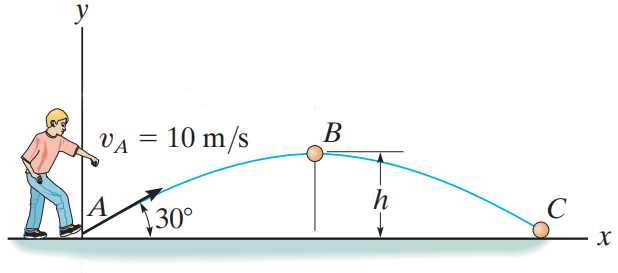
\includegraphics[scale=1.8, height=128pt]{pic2}
			\begin{enumerate}[k]
				\item ចូរសរសេរសមីការគន្លងនៃចលនារបស់គ្រាប់បាល់។
				\item ចូរគណនាចម្ងាយធ្លាក់ $x$ របស់គ្រាប់បាល់ពេលវាធ្លាក់ដល់ចំណុច $C$។\\
				គេឲ្យ $g=10m/s^2$ និង\\ $\cos\frac{\pi}{6}=\frac{\sqrt{3}}{2},~\sin\frac{\pi}{3}=\frac{\sqrt{3}}{2}, \tan\frac{\pi}{6}=\frac{\sqrt{3}}{3}$
			\end{enumerate}
		\end{multicols}
	\end{enumerate}
\newpage
\borderline{\bigg[អត្រាកំណែវិញ្ញាសា រូបវិទ្យា\bigg]}\\
\begin{enumerate}[I]
	\item គណនាបម្លាស់ទីនៃចល័តនោះនៅខណៈ $t=1s$
	\begin{flalign*}
		\text{តាមរូបមន្ត}\quad & \Delta \vec{r}=\vec{r_2}-\vec{r_1}=\Delta \vec{x} + \Delta \vec{y}\\
		\text{ជាម៉ូឌុល}\quad & \Delta r = \sqrt{\left(\Delta x\right)^2+\left(\Delta y\right)^2}\\
		\text{ដោយ}\quad & x_1=\left(3+6t\right)m
		\quad y_1=\left(-5+3t\right)m\\
		\quad & x_2=\left(5+6t\right)m
		\quad y_2=\left(-5-3t\right)m\\
		\text{គេបាន}\quad & \Delta x = x_2-x_1=\left(5+6t\right)-\left(3+6t\right)=2m\\
		\quad & \Delta y = y_2-y_1=\left(-5-3t\right)-\left(-5+3t\right)=-6t(m)\\
		\text{នៅខណៈ}\quad  t=1s & \quad \text{នោះ}\quad   \Delta y = -6(1)=-6m\\
		\text{គេបាន}\quad & \Delta r = \sqrt{\left(2\right)^2+\left(-6\right)^2}=\sqrt{40}=2\sqrt{10}m\\
		\text{ដូចនេះ}\quad & \fbox{$\Delta r = 2\sqrt{10}m$}
	\end{flalign*}
	\item គណនាមាឌឧស្ម័ននីត្រូសែន 
	\begin{flalign*}
	\text{តាមរូបមន្ត}\quad & PV=nRT\\
	\Rightarrow			  \quad & V= \frac{nRT}{P}\\
	\text{ដោយ}\quad & R=8.31J/mol\cdot K\\
	\quad & T=127+273K=400K\\
	\quad & P=2.0\times10^{5}Pa\\
	\quad & m=2.8g\\
	\quad & M\left(N_2\right)=28g/mol\\
	\text{តែ}\quad & n=\frac{m}{M}=\frac{2.8}{28}=0.1mol\\
	\Rightarrow \quad & V=\frac{0.1\times8.31\times400}{2.0\times10^{5}}=1662\times10^{-6}m^{3}\\
	\text{ដូចនេះ}​​\quad & \fbox{$V=1662\times10^{-6}m^{3}$}
	\end{flalign*}
	\item \begin{enumerate}[k]
		\item គណនាល្បឿនដំណាលរលកនៃលំញ័រនេះ
		\begin{flalign*}
		\text{តាមរូបមន្ត}\quad & v=\frac{x}{t}\\
		\text{ដោយ}\quad & x=l=12.0m,\quad t=3.0s\\
		\text{គេបាន}\quad & v=\frac{12.0}{3.0}=4.0m/s\\
		\text{ដូចនេះ}\quad & \fbox{$v=4.0m/s$}
		\end{flalign*}
		\item គណនា
		\begin{flalign*}
		\text{គេមាន}​\quad & y=6\sin\left(100\pi t+ \frac{\pi}{4}\right)\\
		\text{សមីការមានរាង:}\quad & y = a\sin\left(\omega t + \varphi_0\right)
		\end{flalign*}
		\begin{itemize}
			\item អំព្លីទុត
			\begin{flalign*}
			\text{គេបាន}\quad & \fbox{$a=6.0cm$}\\
			\end{flalign*}
			\item មុំផាសដើម
			\begin{flalign*}
			\text{គេបាន}\quad & \fbox{$\varphi_0=\frac{\pi}{4}rad$}\\
			\end{flalign*}
			\item ខួប
			\begin{flalign*}
			\text{គេបាន}\quad & \omega = 100\pi rad/s\\
			\text{តាមរូបមន្ត}\quad & T=\frac{2\pi}{\omega}\\
			\Rightarrow \quad & T=\frac{2\pi}{100\pi}=\frac{1}{50}=\fbox{$0.02s$}\\
			\end{flalign*}
			\item ប្រេកង់
			\begin{flalign*}
			\text{តាមរូបមន្ត}\quad & f=\frac{1}{T}=\frac{1}{\frac{1}{50}}=\fbox{$50Hz$}
			\end{flalign*}
			\item ជំហានរលក
			\begin{flalign*}
			\text{តាមរូបមន្ត}\quad & \lambda = VT\\
			\Rightarrow\quad & \lambda = 4.0\times0.02=\fbox{$0.08m$}\\
			\end{flalign*}
		\end{itemize}
	\end{enumerate}
	\item \begin{enumerate}[k]
		\item កំណត់វុិចទ័រល្បឿន និងវុិចទ័រសំទុះរបស់ភាគល្អិត
		\begin{flalign*}
			\text{តាមរូបមន្ត}\quad & \vec{v}=\frac{d\vec{r}}{dt}\\
			\text{ដោយ}\quad & \vec{r}=\left(4\cos t\vec{i}+4\sin t \vec{j}\right)m\\
			\text{នាំឲ្យ}\quad & \vec{v}=\frac{d\vec{r}}{dt}=\left(4\cos t\vec{i}+4\sin t \vec{j}\right)'=\fbox{$\left(-4\sin t\vec{i}+4\cos t\vec{j}\right)m/s$}
			\\
			\text{តាមរូបមន្ត}\quad & \vec{a}=\frac{d\vec{v}}{dt}\\
			\Rightarrow \quad & \vec{a}=\frac{d\vec{v}}{dt}=\left(-4\sin t\vec{i}+4\cos t\vec{j}\right)'=\fbox{$\left(-4\cos t \vec{i}-4\sin t \vec{j}\right)m/s^2$}\\
		\end{flalign*}
		\item គណនាសំទុះរបស់ភាគល្អិត
		\begin{flalign*}
			\text{គេមាន}\quad & \vec{a}=\left(-4\cos t \vec{i}-4\sin t \vec{j}\right)m/s^2\\
			\text{គេបាន}\quad & a=\sqrt{\left(-4\sin t\right)^2+\left(-4\sin t\right)^2}=\sqrt{\left(-4\right)^2\left(\cos^2t+\sin^2t\right)}=4m/s\quad\text{ព្រោះ​ $\cos^2t+\sin^2t=1$}\\
			\text{ដូចនេះ}\quad & \fbox{$a=4m/s^2$}
		\end{flalign*}
	\end{enumerate}
	\item \begin{enumerate}[k]
		\item កំណត់វិុចទ័រល្បឿនជាអនុគមន៍នៃពេល
		\begin{flalign*}
			\text{តាមរូបមន្ត}\quad & \vec{v}=\frac{d\vec{r}}{dt}\\
			\text{ដោយ}\quad & \vec{r}=3.00\vec{i}-6.00t^2\vec{j}\\
			\text{គេបាន}\quad &\vec{v}=\frac{d\vec{r}}{dt}=\left(3.00\vec{i}-6.00t^2\vec{j}\right)'=0\vec{i}-12.00t\vec{j}\\
			\text{ដូចនេះ}\quad & \fbox{$\vec{v}=0\vec{i}-12.00t\vec{j}$}
		\end{flalign*}
		\item កំណត់វុិចទ័រសំទុះនៃចំណុចរូបធាតុជាអនុគមន៍ពេល
		\begin{flalign*}
			\text{តាមរូបមន្ត}\quad & \vec{a}=\frac{d\vec{v}}{dt}\\
			\text{ដោយ}\quad & \vec{v}=0\vec{i}-12.00t\vec{j}\\
			\Rightarrow\quad & \vec{a}=\frac{d\vec{v}}{dt}=\left(0\vec{i}-12.00t\vec{j}\right)'=-12.00\vec{j}
		\end{flalign*}
		\item ចូរគណនាតម្លៃនៃវុិចទ័រទីតាំង និងវុិចទ័រល្បឿន នៅខណៈ $t=1.00s$
		\begin{flalign*}
			\text{គេមាន}\quad & \vec{r}=3.00\vec{i}-6.00t^2\vec{j}\\
			\text{ដោយ}\quad & t=1.00s\\
			\quad & \vec{r}=3.00\vec{i}-6.00(1.00)\vec{j}=3.00\vec{i}-6.00\vec{j}\\
			\Rightarrow\quad & r=\sqrt{\left(3.00\right)^2+\left(-6.00\right)^2}=\sqrt{9.00+36.00}=\fbox{$3\sqrt{5}m$}\\
			\text{គេមាន}\quad & \vec{v}=0\vec{i}-12.00t\vec{j}\\
			\quad & \vec{v}=0\vec{i}-12.00(1.00)\vec{j}\\
			\Rightarrow \quad & v=\sqrt{\left(0\right)^2+\left(-12.00\right)^2}=\fbox{$12m/s$}
		\end{flalign*}
	\end{enumerate}
	\item \begin{enumerate}[k]
		\item សរសេរសមីការគន្លងនៃចលនារបស់គ្រាប់បាល់
		\begin{flalign*}
			\text{តាមរូបមន្ត}\quad & y=-\frac{1}{2}g\frac{x^2}{v_A^2\cos^2\theta}+x\tan \theta\\
			\text{ដោយ}\quad & g=10m/s^2\\
			\quad & v_A=10m/s\\
			\quad & \theta = 30^\circ=\frac{\pi}{6}rad\\
			\text{គេបាន}\quad & y=-\frac{1}{2}\times10\times\frac{x^2}{\left(10\right)^2\cos^2\frac{\pi}{6}}+x\tan\frac{\pi}{6}=-\frac{1}{15}x^2+\frac{\sqrt{3}}{3}x\\
			\text{ដូចនេះ}\quad & \fbox{$y=-\frac{1}{15}x^2+\frac{\sqrt{3}}{3}x$}
		\end{flalign*}
		\item ចូរគណនាចម្ងាយធ្លាក់ $x$ របស់គ្រាប់បាល់ពេលវាធ្លាក់ដល់ចំណុច $C$
		\begin{flalign*}
			\text{តាមរូបមន្ត}\quad & x=\frac{v_A^2\sin2\theta}{g}\\
			\text{គេបាន}\quad & x= \frac{\left(10\right)^2\sin2\left(\frac{\pi}{6}\right)}{10} = 5\sqrt{3}m\\
			\text{ដូចនេះ}\quad & \fbox{$x=5\sqrt{3}m$}
		\end{flalign*}
	\end{enumerate}
\end{enumerate}
\end{document}